\documentclass[12pt]{amsart}
\usepackage[left=0.5in, right=0.5in, bottom=0.75in, top=0.75in]{geometry}
\usepackage[english]{babel}
\usepackage[utf8x]{inputenc}
\usepackage{amsmath,amssymb,amsthm}
\usepackage{enumerate}
\usepackage{graphicx}

\usepackage[table,xcdraw,dvipsnames]{xcolor}
\usepackage{tikz}
\usepackage{pgfplots}
\usepgfplotslibrary{fillbetween}
\usepackage{booktabs}

\renewcommand{\thesection}{}
\renewcommand{\thesubsection}{\arabic{subsection}}
\renewcommand{\thesubsubsection}{\quad(\alph{subsubsection})}

\begin{document}
\raggedbottom

\noindent{\large OPER 618 - Game Theory and Math Programming %
	- Homework 8 }
\hspace{\fill} {\large B. Hosley}
\bigskip


%%%%%%%%%%%%%%%%%%%%%%%
\setcounter{subsection}{0}
For Questions 1-5, consider the following coalition game:

\begin{center}
	{\renewcommand{\arraystretch}{1.2}
	\begin{tabular}{|c|c|}
		\hline
		\rowcolor[HTML]{C0C0C0} 
		\(S\) 		& \(v(S)\) 	\\ \hline
		$\varnothing$ & $0$ 	\\ \hline
		$\{1\}$ 	& $\alpha$ 	\\ \hline
		$\{2\}$ 	& $0.2$ 	\\ \hline
		$\{3\}$ 	& $0.3$ 	\\ \hline
		$\{1,2\}$ 	& $0.4$ 	\\ \hline
		$\{1,3\}$ 	& $\beta$ 	\\ \hline
		$\{2,3\}$ 	& $0.5$ 	\\ \hline
		$N=\{1,2,3\}$ & $1$ 	\\ \hline
	\end{tabular}}
\end{center}

\subsection{}
\textbf{Game Classification.} 
\textit{For what values of $\alpha$ and $\beta$ is the game superadditive? (Provide a plot of $(\alpha,\beta)$ with the relevant domain shaded.)}


\begin{center}
	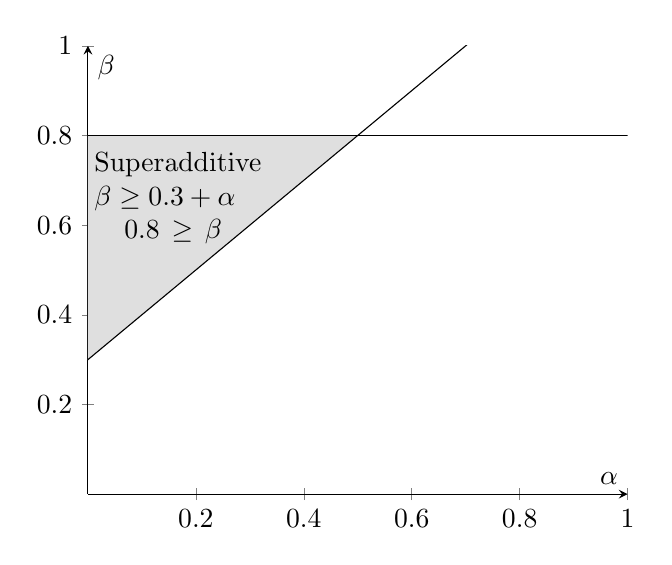
\begin{tikzpicture}
		\begin{axis}[xmin=0, xmax=1, ymin=0, ymax=1, axis x line=middle, axis y line=middle, ylabel=$\beta$, xlabel=$\alpha$]
			\addplot[name path=a]{0.3+x};
			\addplot[]{0.8};
			\addplot[name path=b,domain=0:0.5]{0.8};
			\addplot[gray!25] fill between[of=a and b];
			\node[text width=2cm,align=center] at (axis cs:0.158,0.66) {Superadditive\newline $\beta\geq0.3+\alpha\newline  0.8\geq\beta$};
		\end{axis}
	\end{tikzpicture}
\end{center}



\subsection{}
\textbf{Game Classification.} 
\textit{What additional restrictions, if any, are required on $\alpha$ and/or $\beta$ to ensure the game is convex? (Provide a plot of $(\alpha,\beta)$ with the relevant domain shaded.)}

The only non-redundant constraint is added from $\{1,2\}\cup\{1,3\} \rightarrow 0.6\geq\beta-\alpha$.

\begin{center}
	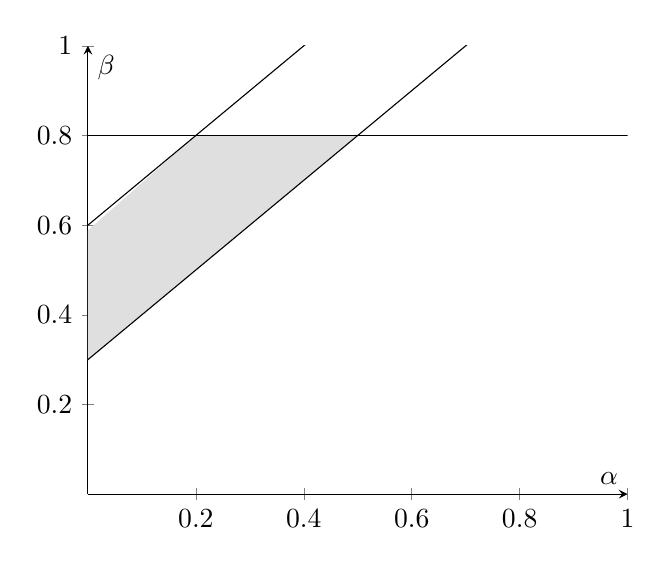
\begin{tikzpicture}
		\begin{axis}[xmin=0, xmax=1, ymin=0, ymax=1, axis x line=middle, axis y line=middle, ylabel=$\beta$, xlabel=$\alpha$]
			\addplot[name path=a]{0.3+x};
			\addplot[]{0.8};
			\addplot[]{0.6+x};
			\addplot[name path=b,domain=0.2:0.5]{0.8};
			\addplot[gray!25] fill between[of=a and b];
			%\node[text width=2cm,align=center] at (axis cs:0.158,0.66) {Superadditive\newline $\beta\geq0.3+\alpha\newline  0.8\geq\beta$};			
		\end{axis}
	\end{tikzpicture}
\end{center}

\subsection{}
\textbf{Shapley Value Allocations.} 
\textit{Calculate each the player’s Shapley value allocations as a function of $\alpha$ and $\beta$. For a convex game (i.e., given your answer to Question 2 above), identify the respective values of $(\alpha,\beta)$ that would maximize each player’s allocation in a grand coalition.}

$\textcolor{blue}{\varphi_1} = \frac{1}{6}\left[ 2\alpha + 0.2 + \beta-0.3 + 2(0.5) \right] = \textcolor{blue}{ \frac{2\alpha+\beta+0.9}{6} \rightarrow (0.5,0.8) } $

$\textcolor{red}{\varphi_2} = \frac{1}{6}\left[ 2(0.2) + 0.4-\alpha + 0.2 + 2(1-\beta) \right] = \textcolor{red}{ \frac{1-\alpha-\beta}{6} \rightarrow (0,0.3) } $

$\textcolor{green}{\varphi_3} = \frac{1}{6}\left[ 2(0.3) + \beta-\alpha + 0.3 + 2(0.6) \right] = \textcolor{green}{ \frac{2.1+\beta-\alpha}{6} \rightarrow \beta-\alpha = 0.6 } $

\begin{center}
	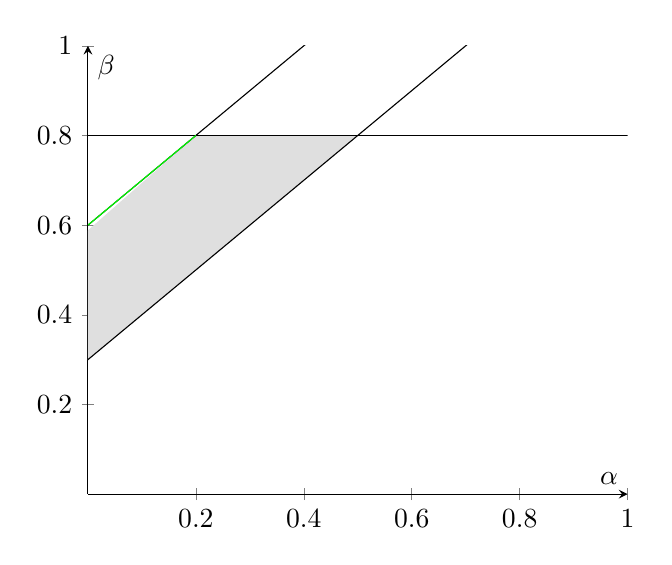
\begin{tikzpicture}
		\begin{axis}[xmin=0, xmax=1, ymin=0, ymax=1, axis x line=middle, axis y line=middle, ylabel=$\beta$, xlabel=$\alpha$]
			\addplot[name path=a]{0.3+x};
			\addplot[]{0.8};
			\addplot[]{0.6+x};
			\addplot[name path=b,domain=0.2:0.5]{0.8};
			\addplot[gray!25] fill between[of=a and b];
			% Optimals
			\draw[thick, blue] (axis cs:0.5,0.8) circle[radius=2];
			\draw[thick, red] (axis cs:0,0.3) circle[radius=2];
			\addplot[domain=0:0.2, color=green]{0.6+x};
		\end{axis}
	\end{tikzpicture}
\end{center}

\subsection{}
\textbf{The Core.} 
\textit{Construct a two-player coalition game with payoffs $v(s),\ \in S \subseteq N$ with an empty core. 
	Show the core is empty. For the sake of this exercise, ensure $v(\{1\}) \neq v(\{2\})$.}

Players: $N={1,2}$

Let's define the characteristic function 
$v:2^{|\mathbb N|} \mapsto \mathbb R$ as \\

\begin{tabular}{c|c}
	$S$ & $v(S)$ \\
	\midrule
	$\varnothing$ & $0$ \\
	$\{1\}$ & $1$ \\
	$\{2\}$ & $2$ \\
	$\{1,2\}$ & $2$ \\
\end{tabular} \\

The core is empty as player 2 has no reason to join the coalition as they gain nothing from doing so.
Additionally, if the coalition was formed and player 2 was willing to join under the condition of receiving
an equal payment, then the remaining payoff is 0 to be split among the other players, 
which would be unreasonable for player 1.

\subsection{}
\textbf{The $\boldsymbol\epsilon$-core.} 
\textit{For the game you created for Question 4, identify the $\epsilon$-core payoff. 
	Discuss the significance of your answer in the context of the game.} \\

From the previous problem we can reformulate the problem with an $\epsilon\geq1$. \\

In the context of this problem that means that there must be a change of at least 1 to any of the values in order for the game to have a non-empty core.
Specifically, the coalition payoff must increase by 1, or either of the individual payoffs must decrease by 1.

\end{document}